\documentclass[12pt]{article}
\usepackage[margin=1.2in]{geometry}
\usepackage{amsmath}
\usepackage{graphicx}
\usepackage{caption}
\usepackage{subcaption}
\begin{document}
\title{COL334 - Assignment 2\\ HTTP}
\author{Akshay Kumar Gupta\\\texttt{2013CS50275} \and  Barun Patra\\\texttt{2013CS10773} \and Haroun Habeeb\\\texttt{2013CS10225}}
\date{}
\maketitle
\noindent
\textbf{Note:} We did the following analysis using HAR and PCAP files of our own. This is because we needed to ensure that the network was the same for comparing goodput of browser and direct request. The network used was Airtel Broadband.\\\\
{\bfseries Q3a.} The source takes the HAR file, the PCAP file and the host IP address as input. The PCAP and HAR files are analysed in conjunction to decide the number of TCP connections per domain and which objects were downloaded on which TCP connection. We only consider those objects whose GET requests exist both in the PCAP and the HAR file to avoid inconsistencies as we found that there are some objects relevant to the page which exist only in the PCAP file and some which exist only in the HAR file.
\\\\
\hspace*{-1.4cm}
{\centering{
{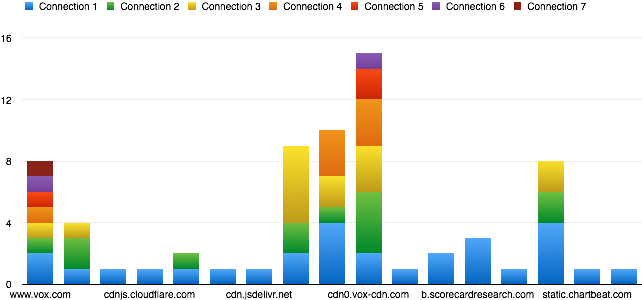
\includegraphics[scale=0.8]{Charts/objectchart.png}
}
}
}
\vspace*{-0.6cm}
\begin{center}Figure 1: No. of objects downloaded on each TCP connection per domain - Nytimes (only some domain names are shown)\end{center}
\hspace*{-1.4cm}
{\centering{
{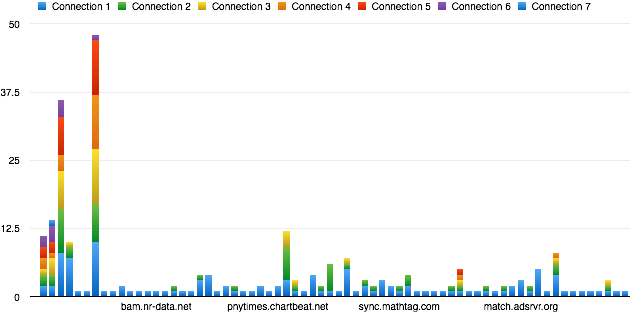
\includegraphics[scale=0.8]{Charts/objectchart1.png}
}
}
}
\vspace*{-0.6cm}
\begin{center}Figure 2: No. of objects downloaded on each TCP connection per domain - Vox (only some domain names are shown)\end{center}
~\\\\
{\centering{
{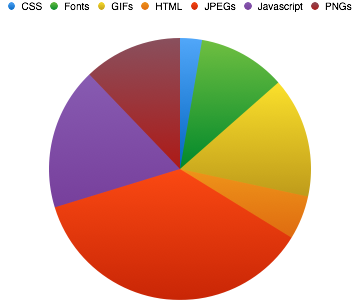
\includegraphics[scale=0.9]{Charts/classchart1.png}
}
}
\begin{center}Figure 3: Classification of objects based on their type - Vox\end{center}
}
~
{\centering{
{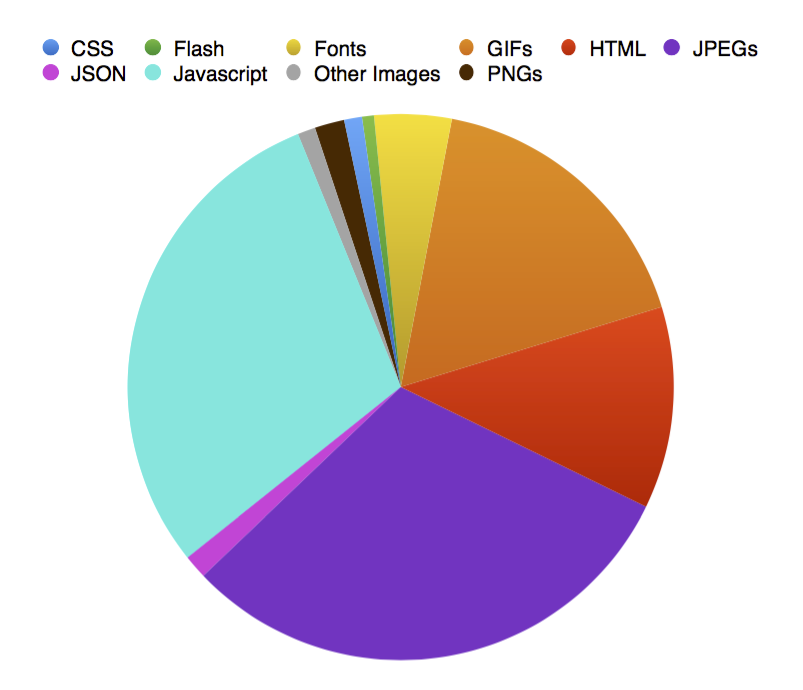
\includegraphics[scale=0.4]{Charts/classchart.png}
}
}
\vspace*{-0.6cm}
\begin{center}Figure 4: Classification of objects based on their type - Nytimes\end{center}
}
~\\
{\bfseries Q3b.} The object and download trees are printed both as terminal output as well as written to a file in the specified format. If the HAR file is named \emph{www.abc.com.har} then the object tree file is named \emph{www.abc.com.objt} and the download tree file is named \emph{www.abc.com.downt}.
\\\\\\
{\bfseries Q3c. i.} The full page load time is calculated using the timing information in the HAR file. The \emph{startedDateTime} field of the first object gives the time for the first DNS request and the maximum of the \emph{startedDateTime} + \emph{time} fields across all objects gives the time the last object was received. \\\\
\textbf{ii.} The observations for DNS query time were rather erratic:
\begin{itemize}
\item For some domains, DNS latency for only the first TCP connection opened is non-zero. This matches our expectation. Eg. \emph{cdnjs.cloudflare.com}, \emph{edge.quantserve.com}
\item For some domains, DNS latency for only one TCP connection is non-zero, but this not the first TCP connection to be opened. A possible reason for this is that many TCP connections opened at almost the same time and DNS query for one of them got answered quickly, and then the rest retrieved the IP from the cache. Eg. \emph{www.vox.com} (Non-zero DNS latency for connection no. 4)
\item For some domains, the DNS latency is 0 (even though the DNS cache was flushed beforehand). In these cases, the only explanation is that DNS resolution was extremely fast. Eg. \emph{a1.nyt.com}, \emph{static01.nyt.com} %TODO reason
\item For some domains, the DNS latency for multiple TCP connections is non-zero. There are two possible reasons for this. One is that the entry was removed from the cache before the subsequent TCP connection was opened. The second reason could be that two TCP connections queried simultaneously when the entry was not in the cache. Eg. \emph{ea-cdn.voxmedia.com}
\end{itemize}
\textbf{iii.} Timing analysis observations:
\begin{itemize}
\item For some TCP connections, the connection establishment time is zero. This probably means that the handshake happened extremely quickly.
\item The sending time was identically zero, which matches expectations.
\item Time for which a TCP connection was active is calculated using the timing information in the HAR file. (Starting time is the \emph{startedDateTime} of the first object and ending time is max(\emph{startedDateTime} + \emph{time}) across all objects downloaded on that connection.)
\item There were a couple of TCP connections on which object downloading times were overlapping based on the timing information in the HAR file, leading to the active percentage being more than one. We currently don't have any intuition as to why this is happening.
\item The maximum goodput when downloaded using a direct GET request was generally greater than the maximum and average goodput when downloaded through the webpage in the case of \emph{www.vox.com} (especially when objects were large), while in the case of \emph{www.nytimes.com}, it was generally smaller. This means that the browser performs well when the object sizes are small (which is the case with nytimes) and worse when object sizes are big (which is the case with vox). One reason for this is the number of parallel objects being downloaded. Our host computer only has four cores so downloads are not truly parallel if more than four objects are being downloaded, so the download time is affected. This is more pronounced for bigger object sizes.
\item For both vox and nytimes, the maximum of the maximum goodput across all TCP connections is much larger than the average goodput across the entire network. This would indicate that the download capacity was not utilized well. However, for most of the TCP connections, the average goodput is similar to and in some cases even greater than the maximum goodput, so for the most part the download capacity was utilized well enough. It is possible that the maximum of the maximum goodput is not representative of the general download capacity and is a outlying case.
\end{itemize}
\hspace*{-1.6cm}
{\centering{
{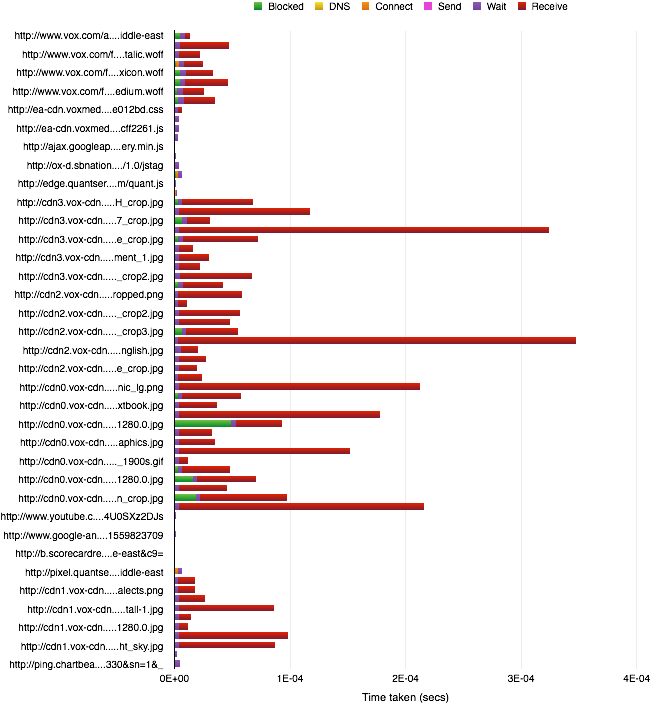
\includegraphics[scale=0.8]{Charts/timeline.png}
}
}
\vspace*{-0.6cm}
\begin{center}Figure 5: Timing data for each object - Vox\end{center}
}
\vspace*{-2cm}
\hspace*{-3cm}
{\centering{
{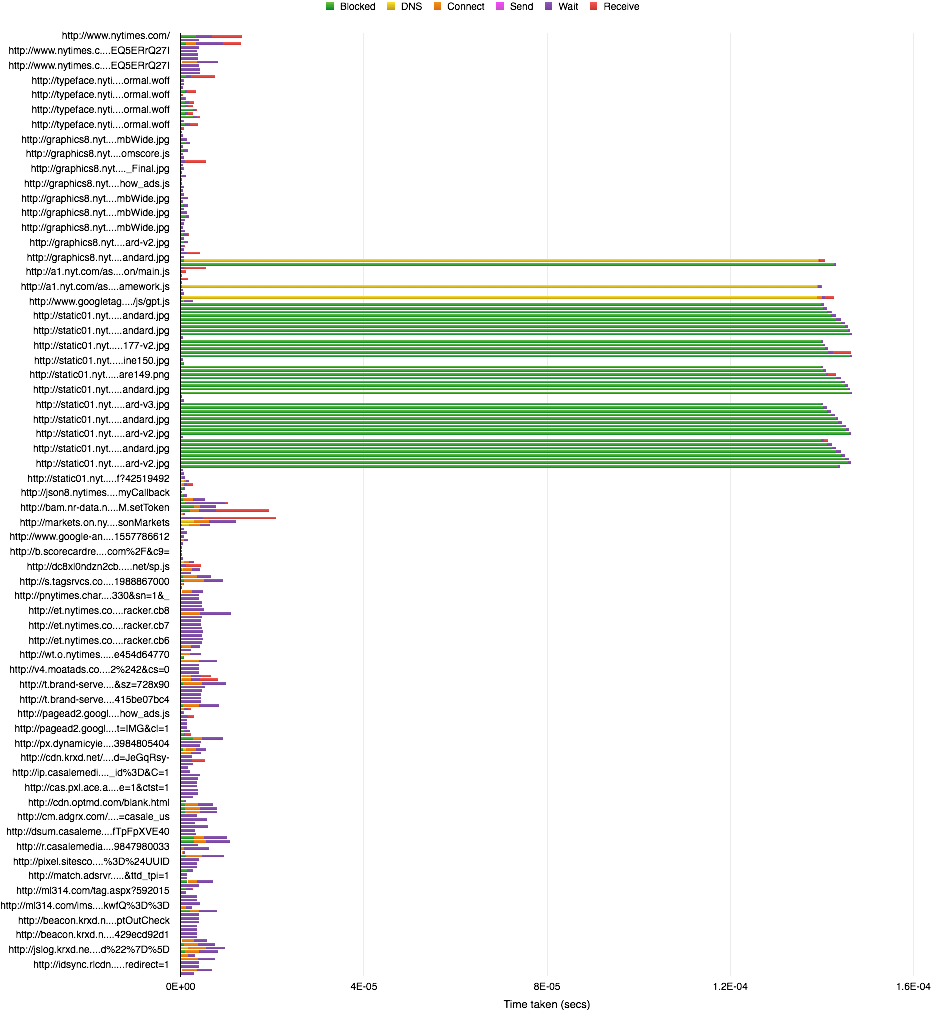
\includegraphics[scale=0.6]{Charts/timeline1.png}
}
}
\vspace*{-0.6cm}
\begin{center}Figure 6: Timing data for each object - Nytimes\end{center}
}
\hspace*{-3cm}
{\centering{
{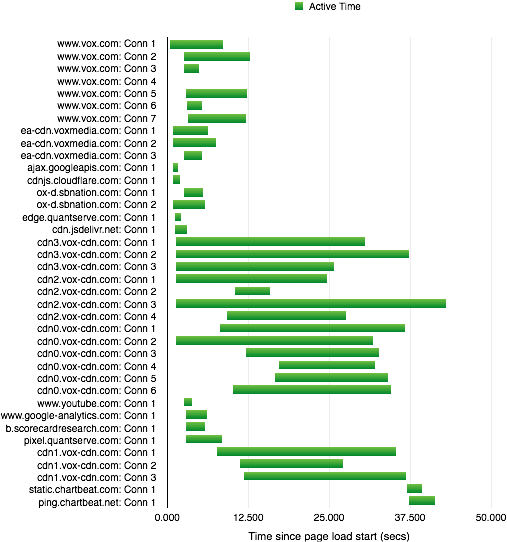
\includegraphics[scale=0.8]{Charts/active_time.png}
}
}
\begin{center}Figure 7: Total active time for each TCP connection - Vox\end{center}
}
\vspace*{-2cm}
\hspace*{-2cm}
{\centering{
{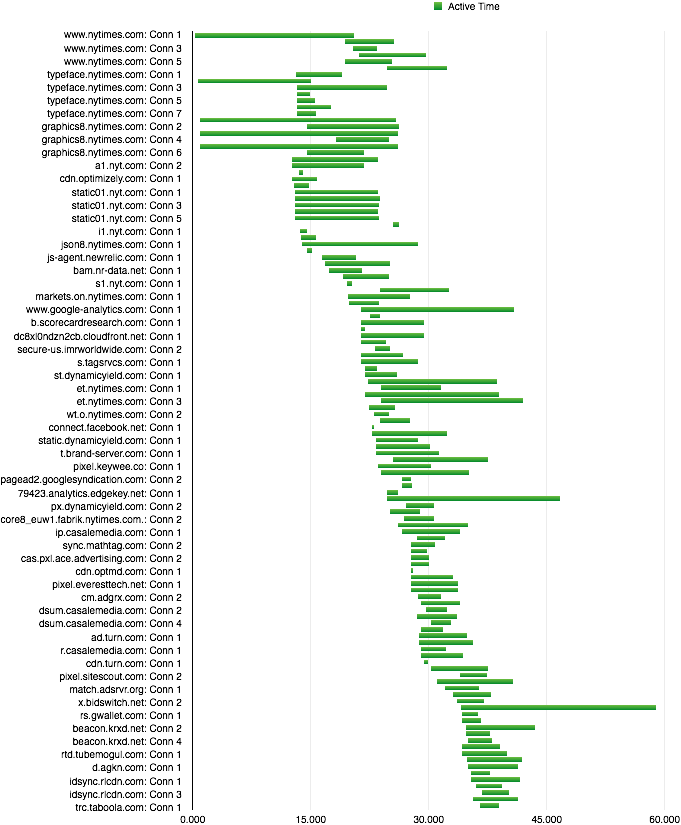
\includegraphics[scale=0.75]{Charts/active_time1.png}
}
}
\begin{center}Figure 8: Total active time for each TCP connection - Vox\end{center}
}
\vspace*{-3cm}
{\centering{
{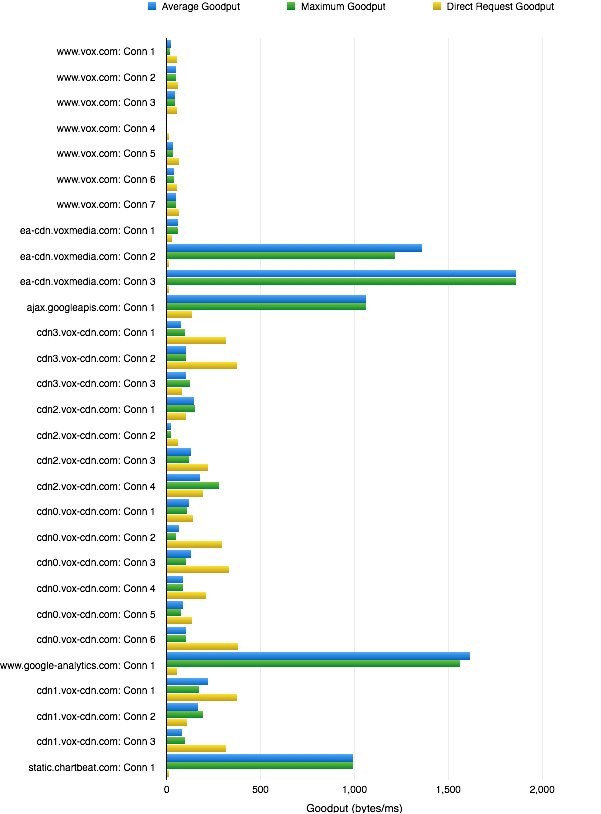
\includegraphics[scale=0.75]{Charts/goodput.png}
}
}
\begin{center}Figure 9: Comparison of maximum and average goodput using browser and maximum goodput using direct request for each TCP Connection - Vox\end{center}
}
\vspace*{-2cm}
\hspace*{-2cm}
{\centering{
{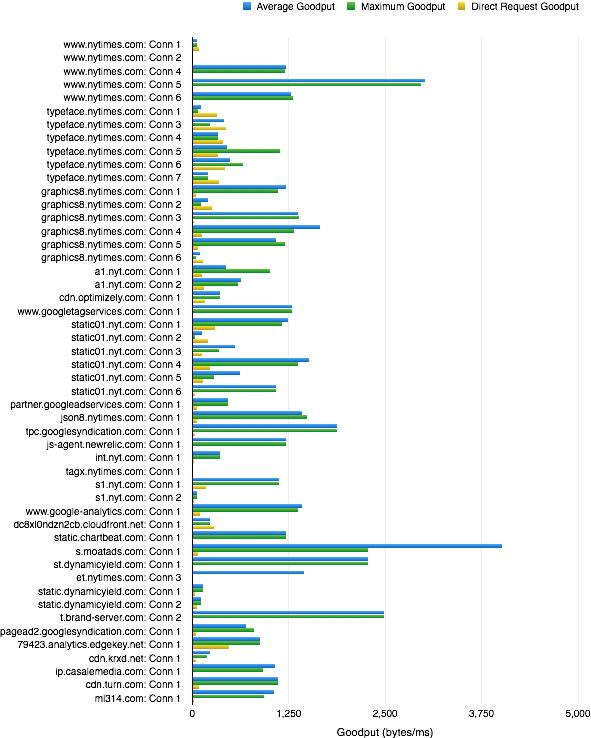
\includegraphics[scale=0.8]{Charts/goodput1.png}
}
}
\begin{center}Figure 10: Comparison of maximum and average goodput using browser and maximum goodput using direct request for each TCP Connection - Nytimes\end{center}
}
~\\
\textbf{iv.} Observations regarding browser imposed caps:
\begin{itemize}
\item We obtained a maximum of 19 parallel TCP connections for nytimes and 16 parallel connections for vox. From this we cannot draw any conclusion about a cap on total number of parallel TCP connections by the browser. 
\item The number of parallel TCP connections to a single domain was at max 6 except for one exception where it was 7. So we can draw a tentative conclusion that the number of parallel TCP connections to a single domain is capped at 6.
\item For the most part no more than 4 objects were downloaded on one TCP connection. But there were a couple of cases where the number of objects downloaded on one TCP connection was as many as 10. So we cannot draw any conclusions about the number of objects downloaded on one connection. However, for comparison purposes in Q4, we will assume this number to be 4. 
\end{itemize}
~\\\textbf{Q3d. i.} We calculated the page load time assuming the objects can be downloaded in parallel on each TCP connection. For vox, the calculated time was 31.432s as compared to the 53s actual time and for nytimes, the calculated time was 15.645s compared to the 68s actual time. The calculated time will always be better because this calculation is a strict relaxation of a browser constraint.
\\\\ \textbf{ii.} We took the maximum goodput of each domain and divided by the total size of objects downloaded on that domain to give us the time taken to receive all the objects of a domain. We took the maximum of these to report the page load time as downloads across domains can work in parallel. This is a good approximation if TCP connection times are within a second or so, which is generally the case.
For vox, the calculated time was 93.767s as compared to the 53s actual time and for nytimes, the calculated time was 6.586s as compared to the 68s actual time. The reason for this is that the maximum goodput is consistently high in the case of nytimes, so always downloading at the maximum goodput will lead to a dramatic increase. In the case of vox, there are a couple of domains for which maximum goodput is very low, leading to a high calculated time and for these domains, parallelisation works better than downloading on a single TCP connection.
\\\\ \textbf{iii.} The calculated time is different for the two cases, because they make two different relaxations on constraints. In the first we make no assumption about the goodput but allow objects on the same connection to be downloaded parallelly and different TCP connections to the same domain to run parallelly as always. In the second case, we assume we can download at the maximum goodput but only on one connection for a domain and serially within that domaian. So calculated times and advantages will be different for both.
\end{document}